\documentclass[letterpaper, 10 pt, conference]{ieeeconf}
\IEEEoverridecommandlockouts
\overrideIEEEmargins
\pdfminorversion=4

\usepackage{cite}
%\usepackage{lcsys}
\usepackage[compact]{titlesec}
\usepackage{amsmath,amssymb,amsfonts}
\usepackage{hyperref}
\usepackage{graphicx}
\usepackage{textcomp}
\usepackage{times}
\usepackage{graphicx}
\usepackage{mathrsfs}
\usepackage{amstext} % Lots of math symbols and environments
\usepackage{algorithm}
\usepackage{algorithmic}
\usepackage{setspace} % For line spacing adjustments
\usepackage{amssymb} % For \qedsymbol
\usepackage{mathtools} 
\usepackage{verbatim}
\usepackage{color}
\usepackage{booktabs} 
\usepackage[font=small]{caption}
\newcommand{\RightComment}[1]{\hfill\(\triangleright\) #1}
\renewcommand{\theenumi}{\alph{enumi}}

\newcommand{\naturals}{\mathbb{N}}
\newcommand{\real}{\mathbb{R}}
\newcommand{\cplx}{\mathbb{C}}
\newcommand{\EX}{\mathbb{E}}
\newcommand{\range}{\mathcal{R}}

% Bibliography setup
% \bibpath is the canonical absolute path to the .bib files. If the bib folder
% moves, update \bibpath below.
%
% BibTeX cannot parse file paths that contain spaces (e.g. "PhD Research"), so
% \bibliography uses \biblink (docs/bib_abs), a local symlink to \bibpath.
% If the symlink is missing, recreate it from the docs/ directory:
%   ln -sfn "/Users/dhruvshah/Library/CloudStorage/OneDrive-UCSanDiego/Documents/Projects/PhD Research/Results_Latex/bib" bib_abs
% Alternatively, compile with -shell-escape and the \write18 line below will
% create the symlink automatically when bib_abs/alias.bib is not found.
\newcommand{\bibpath}{/Users/dhruvshah/Library/CloudStorage/OneDrive-UCSanDiego/Documents/Projects/PhD Research/Results_Latex/bib}
\newcommand{\biblink}{bib_abs}
\IfFileExists{\biblink/alias.bib}{}{\immediate\write18{ln -sfn "\bibpath" "\biblink"}}

\newcommand{\Ac}{\mathcal{A}}
\newcommand{\Bc}{\mathcal{B}}
\newcommand{\Cc}{\mathcal{C}}
\newcommand{\Dc}{\mathcal{D}}
\newcommand{\Ec}{\mathcal{E}}
\newcommand{\Fc}{\mathcal{F}}
\newcommand{\Gc}{\mathcal{G}}
\newcommand{\Hc}{\mathcal{H}}
\newcommand{\Ic}{\mathcal{I}}
\newcommand{\Jc}{\mathcal{J}}
\newcommand{\Kc}{\mathcal{K}}
\newcommand{\Lc}{\mathcal{L}}
\newcommand{\Mc}{\mathcal{M}}
\newcommand{\Nc}{\mathcal{N}}
\newcommand{\Oc}{\mathcal{O}}
\newcommand{\Pc}{\mathcal{P}}
\newcommand{\Qc}{\mathcal{Q}}
\newcommand{\Rc}{\mathcal{R}}
\newcommand{\Sc}{\mathcal{S}}
\newcommand{\Tc}{\mathcal{T}}
\newcommand{\Uc}{\mathcal{U}}
\newcommand{\Vc}{\mathcal{V}}
\newcommand{\Wc}{\mathcal{W}}
\newcommand{\Xc}{\mathcal{X}}
\newcommand{\Yc}{\mathcal{Y}}
\newcommand{\Zc}{\mathcal{Z}}
\newcommand{\abf}{\mathbf{a}}
\newcommand{\bbf}{\mathbf{b}}
\newcommand{\cbf}{\mathbf{c}}
\newcommand{\dbf}{\mathbf{d}}
\newcommand{\fbf}{\mathbf{f}}
\newcommand{\nbf}{\mathbf{n}}
\newcommand{\ubf}{\mathbf{u}}
\newcommand{\vbf}{\mathbf{v}}
\newcommand{\xbf}{\mathbf{x}}
\newcommand{\ybf}{\mathbf{y}}
\newcommand{\zbf}{\mathbf{z}}
\newcommand{\Abf}{\mathbf{A}}
\newcommand{\Bbf}{\mathbf{B}}
\newcommand{\Dbf}{\mathbf{D}}
\newcommand{\Ibf}{\mathbf{I}}
\newcommand{\Kbf}{\mathbf{K}}
\newcommand{\Mbf}{\mathbf{M}}
\newcommand{\Pbf}{\mathbf{P}}
\newcommand{\Qbf}{\mathbf{Q}}
\newcommand{\Rbf}{\mathbf{R}}
\newcommand{\Wbf}{\mathbf{W}}
\newcommand{\alphab}{{\boldsymbol{\alpha}}}
\newcommand{\deltab}{\boldsymbol{\delta}}
\newcommand{\sigmab}{{\boldsymbol{\sigma}}}
\newcommand{\Sigmab}{\boldsymbol{\Sigma}}
\newcommand{\Gammab}{\boldsymbol{\Gamma}}
\newcommand{\xib}{\boldsymbol{\xi}}
\newcommand{\nub}{\boldsymbol{\nu}}
\newcommand{\thetab}{\boldsymbol{\theta}}
\newcommand{\Pib}{\boldsymbol{\Pi}}
\newcommand{\etab}{\boldsymbol{\eta}} 
\newcommand{\phib}{\boldsymbol{\phi}}
\newcommand{\Pf}{\mathfrak{P}}

\newcommand{\EDMD}[3]{\operatorname{EDMD}(#1,#2,#3)}
\newcommand{\Kapprox}{K_{\operatorname{app}}}
\newcommand{\Kedmd}{K_{\operatorname{EDMD}}}
\newcommand{\Kexact}{K_{\operatorname{exact}}}
\newcommand{\Knoisy}{K_{\operatorname{noisy}}}
\newcommand{\Knredmd}{K_{\operatorname{NREDMD}}}
\newcommand{\until}[1]{\{1,\dots,#1\}}
\newcommand{\zuntil}[1]{\{0,\dots,#1\}}
\newcommand{\rank}[1]{\operatorname{rank}(#1)}
\newcommand{\map}[3]{#1:#2 \rightarrow #3}
\newcommand{\deltaxx}{\Delta D^N(X,\Delta X)}
\newcommand{\deltayy}{\Delta D^N(Y,\Delta Y)}
\newcommand{\ybias}{Y_{\bias}^N}
\newcommand{\xbias}{X_{\bias}^N}
\newcommand{\ycov}{Y_{\cov}}
\newcommand{\xcov}{X_{\cov}}
%\newcommand{\dnx}{D^N(X)}
%\newcommand{\dny}{D^N(Y)}
%\newcommand{\tdnx}{\tilde{D}^N(X)}
%\newcommand{\tdny}{\tilde{D}^N(Y)}
\newcommand{\dx}{D(X)}
\newcommand{\dy}{D(Y)}
\newcommand{\psix}{\Psi(X)}
\newcommand{\psixp}{\Psi(X^+)}
\newcommand{\dxs}{D(X_s)}
\newcommand{\dys}{D(Y_s)}
\newcommand{\dxn}[1]{D(X_{#1})}
\newcommand{\dyn}[1]{D(Y_{#1})}
\newcommand{\tdx}{\tilde{D}(X)}
\newcommand{\tdy}{\tilde{D}(Y)}
\newcommand{\Span}{\operatorname{span}}
\newcommand{\blkdiag}{\operatorname{blkdiag}}
\newcommand{\diag}{\operatorname{diag}}
\newcommand{\Tr}{\operatorname{Tr}}
\newcommand{\re}{{\operatorname{re}}}
\newcommand{\im}{{\operatorname{im}}}
\newcommand{\argmin}{\operatorname{argmin}}
\newcommand{\noisy}{{\operatorname{noisy}}}
\newcommand{\bias}{{\operatorname{bias}}}
\newcommand{\exact}{{\operatorname{exact}}}
\newcommand{\cov}{{\operatorname{cov}}}
\newcommand{\rows}{{\operatorname{rows}}}
\newcommand{\cols}{{\operatorname{cols}}}
\newcommand{\rown}{{\operatorname{\sharp rows}}}
\newcommand{\coln}{{\operatorname{\sharp cols}}}
\newcommand{\basis}{{\operatorname{basis}}}
\newcommand{\dist}{{\operatorname{dist}}}
\newcommand{\ssd}{{\operatorname{SSD}}}
\newcommand{\tssd}{{\operatorname{T-SSD}}}
\newcommand{\pred}{{\operatorname{pred}}}
\newcommand{\edmd}{\operatorname{EDMD}}

\newcommand{\fbedmd}[3]{\operatorname{FB-EDMD}(#1,#2,#3)}
\newcommand{\Kfi}[1]{K_{F,#1}}
\newcommand{\Kbi}[1]{K_{B,#1}}
\newcommand{\Mci}[1]{M_{C,#1}}
\newcommand{\ic}{\mathcal{I}_C}


\newcommand{\restr}[2]{#1 \!\! \restriction_{#2}}


\newcommand{\cssd}{C_{\ssd}}
\newcommand{\dssd}{D_{\ssd}}
\newcommand{\dtssd}{D_{\tssd}}
\newcommand{\Kssd}{K_\ssd}
\newcommand{\Ktssd}{K_\tssd}
\newcommand{\ssddx}{\dssd(X)}
\newcommand{\ssddy}{\dssd(Y)}
\newcommand{\dtssdx}{\dtssd(X)}
\newcommand{\dtssdy}{\dtssd(Y)}
\newcommand{\ctssd}{C_{\tssd}}
% command for in-neigbor
%\newcommand{\inn}[1]{{\operatorname{\Nc_{\operatorname{in}}(#1)}}}
\newcommand{\inn}{\Nc_{\operatorname{in}}} 
%\newcommand{\outn}[1]{{\operatorname{\Nc_{\operatorname{out}}(#1)}}}
\newcommand{\outn}{\Nc_{\operatorname{out}}}
\newcommand{\flag}{{\operatorname{flag}}}
%\newcommand{\null}{{\operatorname{null}}}
\newcommand{\symmintersection}{{\operatorname{Symmetric-Intersection}}}
\newcommand{\cmax}{C_{\max}}
%\newcommand{\ctssd}{C_{\operatorname{T-SSD}}}
\newcommand{\mspec}{\operatorname{mspec}}
\newcommand{\mspecnz}{\operatorname{mspec}_{\neq 0}}
\newcommand{\spec}{\operatorname{spec}}
\newcommand{\specnz}{\operatorname{spec}_{\neq 0}}
\newcommand{\sprad}{\operatorname{sprad}}
\newcommand{\rrmse}{\operatorname{RRMSE}}
\newcommand{\rrmsemax}{\operatorname{RRMSE_{\max}}}
\newcommand{\aug}{\operatorname{aug}}
\newcommand{\Faug}{\Fc^{\aug}}
\newcommand{\Taug}{\Tc^{\aug}}
\newcommand{\Kaug}{\Kc^{\aug}}
\newcommand{\innerprod}[2]{\langle #1, #2 \rangle}
\newcommand{\innerprodF}[2]{\langle #1, #2 \rangle_{\Fc}}
\newcommand{\innerprodFaug}[2]{\langle #1, #2 \rangle_{\Faug}}


\newcommand{\longthmtitle}[1]{\mbox{}{\textit{(#1):}}}
\newcommand{\setdef}[2]{\{#1 \; | \; #2\}}
\newcommand{\setdefb}[2]{\big\{#1 \; | \; #2\big\}}
\newcommand{\setdefB}[2]{\Big\{#1 \; | \; #2\Big\}}
\newcommand{\oprocendsymbol}{\hbox{$\square$}}
\newcommand{\oprocend}{\relax\ifmmode\else\unskip\hfill\fi\oprocendsymbol}
\def\eqoprocend{\tag*{$\square$}}

\newtheorem{theorem}{Theorem}[section]
\newtheorem{definition}[theorem]{Definition}
\newtheorem{assumption}[theorem]{Assumption}
\newtheorem{lemma}[theorem]{Lemma}
\newtheorem{remarks}[theorem]{Remarks}
\newtheorem{remark}[theorem]{Remark}
\newtheorem{example}[theorem]{Example}
\newtheorem{corollary}[theorem]{Corollary}
\newtheorem{proposition}[theorem]{Proposition}  
\newtheorem{problem}[theorem]{Problem}

\newcommand{\marginJC}[1]{\marginpar{\color{red}\tiny\ttfamily JC: #1}}
\newcommand{\marginDS}[1]{\marginpar{\color{blue}\tiny\ttfamily DS: #1}}

\newcommand{\R}{\mathbb{R}}
\newcommand{\G}{\mathcal{G}}
\newcommand{\K}{\mathcal{K}}
\newcommand{\A}{\mathcal{A}}
\newcommand{\B}{\mathcal{B}}


\newcommand{\inte}{\operatorname{int}}
\newcommand{\trace}{\operatorname{trace}}
\def\eqoprocend{\tag*{$\bullet$}}

\renewcommand{\baselinestretch}{0.97}
\graphicspath{{figures/}}

\usepackage{multirow}  % Include this package for multi-row functionality
\usepackage{subcaption}  % Include this package for subfigure functionality
\newcommand{\red}[1]{\textcolor{red}{#1}}
\newcommand{\revision}[1]{\textcolor{blue}{#1}}
\renewcommand{\revision}[1]{{#1}}

\allowdisplaybreaks

\def\BibTeX{{\rm B\kern-.05em{\sc i\kern-.025em b}\kern-.08em
    T\kern-.1667em\lower.7ex\hbox{E}\kern-.125emX}}
\pagestyle{empty}

\begin{document}
\title{\LARGE Learning Omega-Limit Partitions from Approximate Koopman Invariants
\thanks{This work was supported by AFOSR Award FA9550-23-1-0740.}}

\author{Dhruv Shah \quad Jorge Cort\'es \thanks{D. Shah and J. Cort\'es
    are with Department of Mechanical and Aerospace Engineering, UC
    San Diego, USA, {\tt\small \{dhshah,cortes\}@ucsd.edu}}}

\maketitle
\thispagestyle{empty}

\begin{abstract}
Nonlinear dynamical systems with multiple omega-limit sets pose a fundamental challenge for global finite-dimensional Koopman modeling with continuous observables. A natural way to address this obstruction is to decompose the state space into forward-invariant regions associated with distinct asymptotic behaviors and to learn a separate Koopman model on each region. This paper studies how to compute such partitions from data. We establish conditions under which Koopman invariant observables, namely eigenfunctions associated with the unit eigenvalue, characterize the stationary partition induced by omega-limit sets. Building on this characterization, we develop an algorithm for extracting partitions from approximate invariant observables learned from data. Numerical examples show that the recovered partitions capture the relevant asymptotic regions and support multiple local linear Koopman models with improved long-horizon prediction.
\end{abstract}

\section{Introduction}
The Koopman operator provides a linear representation of nonlinear dynamics by lifting the evolution from the state space to a space of observable functions. Although the state-space dynamics may be nonlinear, the Koopman operator acts linearly by composition with the flow or map, enabling spectral methods for analysis, prediction, estimation, and control. This perspective has become increasingly influential in data-driven dynamical systems because it offers a principled way to combine nonlinear modeling with linear systems tools. Dynamic mode decomposition (DMD), extended dynamic mode decomposition (EDMD), kernel methods, and neural-network-based Koopman embeddings have made Koopman-theoretic ideas computationally accessible across fluid mechanics, robotics, control, and machine learning \cite{BOK:31,IM:05,MB-RM-IM:12,MOW-IGK-CWR:15,BL-JNK-SLB:18}. The central promise is that, after a suitable change of observables, nonlinear trajectories can be propagated, analyzed, or controlled using finite-dimensional linear models.

Despite this promise, finite-dimensional Koopman modeling has fundamental limitations. In particular, nonlinear systems with multiple omega-limit sets cannot, in general, be represented by a single continuous, finite-dimensional, one-to-one linear immersion. Recent impossibility results show that, under mild assumptions, continuous immersions into finite-dimensional linear systems collapse distinct omega-limit sets and therefore fail to provide globally injective Koopman embeddings \cite{ZL-NO-EDS:25}. This obstruction helps explain a recurring empirical phenomenon: global Koopman models trained with smooth or continuous dictionaries may blur basin boundaries, miss discontinuous invariant coordinates, or produce long-term predictions that remain accurate only on restricted regions of the state space.

A natural way to avoid this obstruction is to abandon the requirement of a single global finite-dimensional model and instead decompose the state space into dynamically meaningful invariant regions. Once such regions are known, one can learn a separate Koopman model on each region, obtaining local linear descriptions that respect the distinct asymptotic behaviors of the nonlinear system. Another advantage of this approach is that since the state-space will be partitioned in forward invariant regions, no switching is needed to transition between different models i.e. given an initial condition, the model to use is determined by the partition and the model is used for the entire duration of the simulation. This idea has appeared in several forms. Williams et al. \cite{MOW-IGK-CWR:15} used EDMD eigenfunctions to identify the basins of attraction of the Duffing oscillator and then applied EDMD separately on the resulting subdomains. Nandanoori et al. \cite{SPN-SS-EY:20} proposed using spectral properties of a data-driven Koopman operator to identify invariant subsets of the phase space and introduced a phase-space stitching construction in which local Koopman operators are assembled into a block-diagonal global operator using characteristic functions of the invariant regions. Their framework assumes either access to a global Koopman operator whose eigenvectors reveal the invariant regions or prior knowledge of the local invariant sets needed to construct the characteristic functions used for stitching. In contrast, the present paper formulates the target object as the omega-limit partition and develops a data-driven algorithm for learning this partition directly from approximate Koopman invariants. The local Koopman models are then constructed after the partition has been recovered, rather than assuming the partition in advance.

Local Koopman constructions have also been used for data-driven control, where separate linear models are learned in regions whose dynamics are more amenable to finite-dimensional approximation \cite{GM-MC-XT-TM:19}. More recently, Pan and Duraisamy \cite{SP-KD:24} studied Koopman lifting and reconstruction for systems with multiple invariant sets, emphasizing the role of basin-dependent eigenfunctions and symmetry in data-efficient learning. These works suggest that multiple Koopman models are often the appropriate modeling object for systems with multiple attractors or omega-limit sets, but they do not provide a general data-driven procedure, with supporting theory, for learning the underlying omega-limit partition itself.

Other related work includes the problem of building ergodic partitions for measure-preserving dynamical systems. Mezi{\'c} and Wiggins \cite{IM-SW:99} introduced a method for constructing ergodic partitions through level sets of time-averaged observables. Levnaji{\'c} and Mezi{\'c} \cite{ZL-IM:10} developed this idea computationally through mesochronic plots, which approximate ergodic partitions by computing time averages of observables along trajectories. Susuki and Mezi{\'c} \cite{YS-IM:09} extended the ergodic-partition framework to continuous-time dynamical systems and demonstrated its utility for transient stability analysis in power systems. These works are conceptually close to the present paper because, in the measure-preserving setting, time-averaged observables are invariant almost everywhere whenever the averages exist, and therefore define elements of the unit-eigenvalue eigenspace of the Koopman operator. The objective and setting here are different: the ergodic-partition literature primarily studies measure-preserving or recurrent dynamics and seeks invariant components on which the dynamics is ergodic, whereas this paper does not assume measure preservation and focuses on systems with multiple omega-limit sets. Rather than computing long-time averages, we recover invariant coordinates directly from data by solving a generalized eigenvalue problem for approximate Koopman invariants, and then use the resulting partition to learn multiple local Koopman models.

Another related direction uses Koopman eigenfunctions to identify basins of attraction and stability boundaries. In particular, Umathe and Vaidya \cite{BU-UV:23} characterize the stability boundary of a nonlinear autonomous system using the zero-level set of a Koopman eigenfunction associated with an unstable equilibrium on the boundary. This is a special case of our work: their goal is to recover the separatrix associated with the region of attraction of a given stable equilibrium, while our goal is to recover the full omega-limit partition associated with all distinct asymptotic behaviors. 

Our contributions are as follows. We study autonomous dynamical systems with multiple omega-limit sets and define the omega-limit partition induced by the equivalence relation \(x\sim_\omega y\) if and only if \(\omega(x)=\omega(y)\). We formulate recovery of this partition as a Koopman-invariant-observable problem, connecting asymptotic state-space structure with the \(\lambda=1\) eigenspace of the Koopman operator. We show that invariant Koopman observables induce stationary partitions through their level sets, that continuous invariant observables induce partitions that are coarser than the omega-limit partition, and that equality holds when these observables separate distinct omega-limit cells. We then move from exact invariants to approximate invariants learned from data. Under approximation assumptions on the dictionary, we show that approximate invariant observables can separate distinct omega-limit cells outside a small exceptional set, provided the dictionary approximates the indicator functions of the omega-limit cells. This result motivates a practical algorithm: solve a generalized eigenvalue problem to compute approximate invariant observables, construct an initial fine partition by clustering the data in the resulting invariant-observable coordinates, and merge spurious fragments using transition-based and value-space criteria. The resulting partition is then used to learn multiple local Koopman models, one on each recovered omega-limit region. Numerical examples on systems with multiple equilibria and multiple limit cycles demonstrate that the proposed method recovers meaningful asymptotic regions and improves long-term prediction relative to a single global model.
\section{Preliminaries}

In this section\footnote{We use the following notation. Let $\real^n$
  denote the $n$-dimensional Euclidean space and
  $\mathcal{X} \subseteq \real^n$ the state space. For a matrix
  $M \in \real^{m \times n}$, we denote its range (column space) by
  $\mathcal{R}(M)$, its rank by $\rank{M}$, and its Moore-Penrose
  pseudoinverse by $M^\dagger$. For subspaces
  $\Uc, \Vc \subseteq \real^n$, we denote the orthogonal projection
  onto $\Uc$ by $\Pc_{\Uc}$, and the orthogonal complement by
  $\Uc^\perp$. We write $\Uc \oplus \Vc$ to denote the orthogonal
  direct sum when $\Uc \cap \Vc = \{0\}$ and $\Uc \perp \Vc$. For a
  Hilbert space $\Hc$ with inner product
  $\langle \cdot, \cdot \rangle_{\Hc}$ and induced norm
  $\|\cdot\|_{\Hc}$, subspaces of observables are denoted by
  calligraphic letters (e.g., $\Sc, \Vc$). We use $\text{span}(\cdot)$
  to denote the linear span and $\text{dim}(\cdot)$ to denote
  dimension. The distance from a point $x$ to a subspace $\Uc$ is
  $\text{dist}(x, \Uc) = \inf_{u \in \Uc} \|x - u\|$. We denote
  $i = 1 , \dots, k$ as $i \in [k]$ for brevity.  }, we review the
Koopman operator and the partition concepts used
throughout the paper.

\subsection{The Koopman Operator}
Following~\cite{AM-YS-IM:20}, consider a discrete-time dynamical
system on the state space $\mathcal{X} \subseteq \mathbb{R}^n$
described by a map $T: \mathcal{X} \to \mathcal{X}$:
\begin{equation}\label{eqn:sys_dynamics}
  x^+ = T(x), \quad x \in \mathcal{X}.
\end{equation}
The Koopman operator $\mathcal{K}: \mathcal{F} \to \mathcal{F}$ is an
infinite-dimensional linear operator that acts on a space of
real-valued observables
$\mathcal{F} \ni \psi: \mathcal{X} \to \mathbb{R}$ by composing them
with the dynamics: $(\mathcal{K}\psi)(x) = \psi(T(x))$. We assume that the function space $\mathcal{F}$ is closed under composition with $T$. The linearity of $\mathcal{K}$ enables the use of spectral methods: the eigenvalues and eigenfunctions of $\mathcal{K}$ encode the long-term asymptotic behavior of the system through the evolution of observable
functions. 

We equip the space of observables
$\mathcal{F}$ with a Hilbert space structure by defining an inner
product $\langle \cdot, \cdot \rangle_{\mathcal{F}}$ and the
associated norm $\|\cdot\|_{\mathcal{F}}$. A common choice is the
$L_2$-space with respect to a probability measure $\mu$ on
$\mathcal{X}$. 


\subsection{Partitions and Stationary Partitions}

We introduce some definitions related to partitions that will be used to formalize the problem statement and subsequent results.

\begin{definition}[Partition, measurable partition \cite{IM-SW:99}]\label{def:partition}
A family $\Pc=\{C_\alpha\}_{\alpha\in A}$ of disjoint nonempty subsets of $\Xc$ whose union is $\Xc$ is called a \emph{partition} of $\Xc$. Each $C_\alpha$ is called an \emph{element} (or \emph{cell}) of $\Pc$. A subset $D\subseteq\Xc$ is a \emph{$\Pc$-set} if it is a union of elements of $\Pc$.

Assume $\Xc$ is equipped with a $\sigma$-algebra $\Bc$ and a probability measure $\mu$. The partition $\Pc$ is \emph{measurable} if there exists a countable family $\Delta=\{D_i\}_{i\in\naturals}\subseteq\Bc$ such that every $D_i$ is a $\Pc$-set, and for every pair of elements $C_1,C_2\in\Pc$ there exists $D_j\in\Delta$ with $C_1\subseteq D_j$ and $C_2\subseteq D_j^c$. The family $\Delta$ is called a \emph{basis} for $\Pc$.
\oprocend
\end{definition}

A partition $\Pc_1$ is \emph{finer} than a partition $\Pc_2$, written $\Pc_1\succeq\Pc_2$, if every element of $\Pc_2$ is a $\Pc_1$-set. Equivalently, every $\Pc_2$-set is a $\Pc_1$-set. In this case, $\Pc_2$ is \emph{coarser} than $\Pc_1$. We omit the partition index when it causes no confusion.


\begin{definition}[Stationary partition]
A measurable partition $\mathcal P=\{C_\alpha\}_{\alpha\in A}$ of $\Xc$ is called a stationary partition if every $C_\alpha$ is forward invariant: $T(C_\alpha)\subseteq C_\alpha, \,\, \forall \alpha\in A.$
\oprocend
\end{definition}

\begin{remark}[Non-uniqueness]
Stationary partitions are not unique. We can combine cells of a stationary partition to obtain a coarser stationary partition. For example, if $\{C_1, C_2\}$ is a stationary partition, then $\{\Xc\} = \{C_1 \cup C_2\}$ is also a stationary partition. In general, any partition that can be obtained by merging cells of a stationary partition is itself stationary.
\oprocend
\end{remark}


\subsection{Omega-limit sets and the omega-limit partition}

We talk about the basic properties of omega-limit sets. This will help us to construct the omega-limit partition which is a unique stationary partition of the state space $\Xc$ that captures the asymptotic behavior of the system.

\marginDS{I dont think Khalil is the correct reference here.}

\begin{definition}[Omega-limit set \cite{HK:02}]
The omega-limit set of $x\in\Xc$, denoted $\omega(x)$ is defined as
\begin{equation}
    \omega(x)
    :=
    \left\{y\in\Xc:\exists\, n_j\to\infty \text{ such that } T^{n_j}(x)\to y\right\},
\end{equation}
i.e. it is the set of all accumulation points of the forward orbit of $x$.
\end{definition}
\smallskip

\begin{lemma}[Basic properties of omega-limit sets \cite{HK:02}]
For every $x\in\Xc$, the set $\omega(x)$ is nonempty, compact, and invariant in the sense that
\begin{equation}
    T(\omega(x)) = \omega(x).
\end{equation}
Furthermore, for every $x\in\Xc$ and integer $k\geq 0$, we have $\omega(T^k x)=\omega(x)$.
\oprocend
\end{lemma}


\section{Problem Statement}
Consider a discrete-time autonomous dynamical system
\begin{equation}
\label{eq:dynamics}
    x^+ = T(x), \qquad x \in \Xc,
\end{equation}
where $\Xc$ is the state space and $T:\Xc\to \Xc$ is the dynamics map. Unless stated otherwise, $\Xc$ is a compact metric space, $T:\Xc\to\Xc$ is continuous, and $\Xc$ is forward invariant under the dynamics. The system may have multiple omega-limit sets, corresponding to distinct asymptotic behaviors.

The goal of this paper is to learn a distinguished stationary partition, namely the omega-limit partition $\mathcal P_\omega$ in Definition \ref{def:omega_limit_partition}, from data.
\begin{definition}[Omega equivalence relation]
Define a relation $\sim_\omega$ on $\Xc$ by $    x\sim_\omega y
    \quad\Longleftrightarrow\quad
    \omega(x)=\omega(y)$, where $\omega(x)$ is the omega-limit set of $x$.
The equivalence class of $x$ is $R_\omega(x)
    :=
    \{y\in\Xc:\omega(y)=\omega(x)\}.$
\oprocend
\end{definition}

\smallskip
It is straightforward to verify that $\sim_\omega$ is an equivalence relation, so the equivalence classes $R_\omega(x)$ form a partition of $\Xc$. The following definition gives this partition a name.

\begin{definition}[Omega-limit partition]\label{def:omega_limit_partition}
The omega-limit partition $\Pc_{\omega}$ is the collection of equivalence classes
\begin{equation}
    \mathcal P_\omega
    :=
    \{R_\omega(x):x\in\Xc\}.
\end{equation}
The basic properties of omega-limit sets imply that $\mathcal P_\omega$ is a stationary partition and unique. \oprocend
\end{definition}
\smallskip

This property motivates our interest in learning $\mathcal P_\omega$ from data: once the cells are known, one can learn local linear Koopman models on each cell that capture the distinct asymptotic behaviors of the system.

\textbf{Problem statement:}
We assume access to snapshot pairs $\{(x_i, y_i)\}_{i=1}^N$ with $y_i = T(x_i)$, together with a dictionary of candidate observables $\Psi = \{\psi_1, \dots, \psi_s\}$ spanning a subspace $\Sc$. Our objective is to extract from the data a partition $\hat{\mathcal P}$, built from approximate Koopman invariants, that approximates the true omega-limit partition $\mathcal P_\omega$.

The rest of this paper is organized as follows. Section~\ref{sec:invariant_observables} establishes the connection between invariant observables and the omega-limit partition. Section~\ref{sec:approximate_invariants} studies approximate invariants and their ability to approximate the true omega-limit partition. Section~\ref{sec:post_processing_partition} presents a practical algorithm for learning the omega-limit partition from data, and Section~\ref{sec:numerical_examples} illustrates the approach with numerical examples.

\section{Invariant Observable Partitions}
\label{sec:invariant_observables}

Our first step towards solving the problem is to establish connections between invariant observables and the omega-limit partition. Throughout this paper we assume that the function space $\Fc$ is closed under composition with $T$, and is comprised of continuous real-valued functions on $\Xc$. 

\begin{definition}[Invariant observables]
Elements of the $\lambda=1$ eigenspace $E_{\text{inv}}(K)$ of the Koopman operator are invariant observables of \eqref{eq:dynamics}. Formally,
\begin{equation*}
    E_{\text{inv}}(K)
    :=
    \{f\in\Fc:Kf=f\}. \eqoprocend
\end{equation*}
\end{definition}
\smallskip

Next, we describe how invariant observables induce stationary partitions through their level sets.

\begin{proposition}\longthmtitle{Partitions induced by invariant observables}
Let $f\in E_{\text{inv}}(K)$. For $c\in\R$, define the level set
\begin{equation}
    C_c^f := \{x\in\Xc:f(x)=c\}.
\end{equation}
Then each nonempty level set $C_c^f$ is forward invariant. Consequently, the collection of nonempty level sets $ \{C_c^f : c \in \R\} $ of $f$ is a stationary partition of $\Xc$.
\end{proposition}

\begin{proof}
Fix $c\in\R$ and suppose $x\in C_c^f$. Then $f(x)=c$. Since $f$ is invariant, $f \circ T (x)=f(x)=c$. Therefore $T(x)\in C_c^f$ and $T(C_c^f)\subseteq C_c^f$. The nonempty level sets of any function are pairwise disjoint and cover $\Xc$. Since each nonempty level set is forward invariant and each $C_c^f$ is a measurable set, the collection of nonempty level sets is a stationary partition. 
\end{proof}

Next, this is extended to families of invariant observables, which induce partitions through their joint level sets.

\begin{proposition}\longthmtitle{Partition induced by a family of invariant observables}
Let $\mathcal A\subseteq E_{\text{inv}}(K)$ be any family of invariant observables. Define the equivalence relation
\begin{equation}
    x\sim_{\mathcal A} y
    \quad\Longleftrightarrow\quad
    f(x)=f(y)\quad\text{for every } f\in\mathcal A.
\end{equation}
The partition induced by $\mathcal A$ is $\mathcal P_{\mathcal A}:=\{[x]_{\mathcal A}:x\in\Xc\}$, where
\begin{equation}
    [x]_{\mathcal A}:=\{y\in\Xc:f(y)=f(x)\;\forall f\in\mathcal A\}.
\end{equation}
Then, for any $\mathcal A\subseteq E_{\text{inv}}(K)$, the partition $\mathcal P_{\mathcal A}$ is stationary.
\end{proposition}

\begin{proof}
The relation $\sim_{\mathcal A}$ is an equivalence relation, so its equivalence classes form a partition of $\Xc$. Fix a cell $[x]_{\mathcal A}$ and let $y\in[x]_{\mathcal A}$. Then, for every $f\in\mathcal A$, we have $f(y)=f(x).$ Since each $f\in\mathcal A$ is invariant,
\begin{equation}
    f \circ T (y)=f(y)=f(x).
\end{equation}
Thus $T(y)\in[x]_{\mathcal A}$. Hence each cell is forward invariant, so $\mathcal P_{\mathcal A}$ is a stationary partition.
\end{proof}

\begin{comment}

The natural function space for comparison with omega-limit sets is the space of continuous invariant observables
\begin{equation}
    E_{\text{inv}}^c(K) := E_{\text{inv}}(K)\cap C(\Xc;\real).
\end{equation}
Here $C(\Xc;\real)$ denotes the space of continuous real-valued functions on $\Xc$.

\begin{lemma}\longthmtitle{Continuous invariant observables are constant on omega-limit sets}
Let $f\in E_{\text{inv}}^c(K)$. If $z\in\omega(x)$, then $f(z)=f(x)$.
\label{lemma:cts_observables_constant}
\end{lemma}

\begin{proof}
Since $z\in\omega(x)$, there exists a sequence $n_j\to\infty$ such that
$T^{n_j}(x)\to z$. Because $f$ is invariant, we have $f(T^n (x))=f(x)$ for every $n\geq 0$. Since $f$ is continuous and $T^{n_j}(x)\to z$,
\begin{equation}
    f(z)=\lim_{j\to\infty}f(T^{n_j}(x))=f(x).
\end{equation}
This proves the claim.
\end{proof}

\begin{theorem}\longthmtitle{Continuous invariant-observable partition is coarser than the omega-limit partition}
Let $\mathcal P_{\Ac^c}$ be the partition induced by a family of continuous invariant observables $\Ac^c\subseteq E_{\text{inv}}^c(K)$. Then
\begin{equation}
    x\sim_\omega y
    \quad\Longrightarrow\quad
    x\sim_{\Ac^c} y.
\end{equation}
Equivalently, every omega-limit cell is contained in a cell of $\mathcal P_{\Ac^c}$. Thus $\mathcal P_{\Ac^c}$ is coarser than, or equal to, $\mathcal P_\omega$.
\end{theorem}

\begin{proof}
Assume $x\sim_\omega y$, so $\omega(x)=\omega(y)$. Let $f\in \Ac^c\subseteq E_{\text{inv}}^c(K)$ be arbitrary. Since $\omega(x)$ is nonempty, choose $z\in\omega(x)=\omega(y)$. By Lemma \ref{lemma:cts_observables_constant} applied to the pair $(x,z)$ and $(y,z)$, we have
\begin{equation*}
    f(z)=f(x) \quad \text{and} \quad f(z)=f(y).
\end{equation*}
Therefore $f(x)=f(y)$. Since this holds for every $f\in \Ac^c$, we have $x\sim_{\Ac^c}y$. Hence every $\sim_\omega$ equivalence class is contained in a $\sim_{\Ac^c}$ equivalence class.
\end{proof}

Our next result gives a necessary and sufficient condition for the two partitions $\mathcal P_{\Ac^c}$ and $\mathcal P_\omega$ to be equal.

\begin{lemma}[Equality criterion]
The two partitions $\mathcal P_{\Ac^c}$ and $\mathcal P_\omega$ are equal if and only if $\Ac^c$ separates distinct omega-limit fibers; that is, whenever $\omega(x)\neq\omega(y)$, there exists an observable $f\in\Ac^c$ such that $f(x)\neq f(y)$.
\end{lemma}

\begin{proof}
First suppose $\mathcal P_{\Ac^c}=\mathcal P_\omega$. Let $x,y\in\Xc$ satisfy $\omega(x)\neq\omega(y)$. Then $x$ and $y$ lie in different cells of $\mathcal P_\omega$. Since the two partitions are equal, $x$ and $y$ also lie in different cells of $\mathcal P_{\Ac^c}$. By the definition of $\mathcal P_{\Ac^c}$, this means it is not true that $f(x)=f(y)$ for every $f\in\Ac^c$. Hence there exists $f\in\Ac^c$ such that $f(x)\neq f(y)$. Thus $\Ac^c$ separates distinct omega-limit fibers.

Conversely, suppose $\Ac^c$ separates distinct omega-limit fibers. We already know from the previous theorem that
\begin{equation}
    x\sim_\omega y \implies x\sim_{\Ac^c} y.
\end{equation}
It remains to prove the reverse implication. Suppose $x\sim_{\Ac^c} y$. If $\omega(x)\neq\omega(y)$, then by the separation assumption there exists $f\in\Ac^c$ such that $f(x)\neq f(y)$, contradicting $x\sim_{\Ac^c}y$. Therefore $\omega(x)=\omega(y)$, i.e., $x\sim_\omega y$. Thus
\begin{equation}
    x\sim_{\Ac^c} y \implies x\sim_\omega y.
\end{equation}
Combining the two implications gives equality of the equivalence relations and hence equality of the partitions.
\end{proof}
\end{comment}


\section{Approximate invariant observable partitions}
\label{sec:approximate_invariants}
We now turn to the data-driven setting. Here, the aim is to extract a partition $\Pc_{\epsilon}$ from approximate invariant observables learned from data so that $\Pc_{\epsilon}$ can be coarsened into an approximation of the true omega-limit partition $\mathcal P_\omega$. Recall that we have a dictionary of continuous functions $\Psi = \{\psi_1, \dots, \psi_s\}$ spanning a subspace $\Sc$. Given $\epsilon > 0$, define the set of $\epsilon$-invariant observables in $\Sc$ by
\begin{equation}
    E_{\text{inv}}^{\epsilon}(\Sc) := \{f\in\Sc: \| Kf - f \| \leq \epsilon \|Kf\| \}
\end{equation}

The partition induced by $E_{\text{inv}}^{\epsilon}(\Sc)$ is $\mathcal P_{\epsilon} := \{[x]_{\epsilon}: x \in \Xc\}$, 
\begin{equation}
    \text{where } [x]_{\epsilon} := \{y \in \Xc: f(y) = f(x) \,\, \forall \,\, f \in E_{\text{inv}}^{\epsilon}(\Sc)\}.
\end{equation}
Unlike the exact invariant-observable partitions of the previous section, $\Pc_{\epsilon}$ need not be stationary because the observables in $E_{\text{inv}}^{\epsilon}(\Sc)$ are only approximately invariant. The next theorem gives conditions under which $\Pc_{\epsilon}$ refines $\mathcal P_\omega$ outside a small exceptional set. Thus, the cells of $\Pc_{\epsilon}$ can be merged to recover the coarser omega-limit partition.

\begin{theorem}\longthmtitle{Approximate invariant observables separate omega-limit cells outside a small set}
Suppose the omega-limit partition is finite and measurable:
\begin{equation}
    P_\omega=\{C_1,\dots,C_q\},\,\, \text{with }\mu(C_i)>0,
    \,\, i \in [q]  
\end{equation}
Let $\chi_i:=\mathbf{1}_{C_i}$ be the indicator function of $C_i$. Assume that for each $i \in [q]$, there exist $s_i\in \Sc$, $\delta_i>0$, and $\beta_i \geq 0$ s.t.
\begin{align}
    \|{s_i-\chi_i}\|_{L^2(\mu)} &\leq \delta_i,\
    \|{K(s_i-\chi_i)}\|_{L^2(\mu)} \leq \beta_i\delta_i, \label{eqn:approx_indicator} \\  
    \beta_i \delta_i &< \sqrt{\mu(C_i)}, \,\,
    \frac{(\beta_i+1)\delta_i}
    {\sqrt{\mu(C_i)}-\beta_i\delta_i}
    \leq \varepsilon. \label{eq:epsilon_condition}
\end{align}
Then the functions $s_i$ are $\epsilon$-invariant observables, i.e.,
\begin{equation}
s_i\in E_{\text{inv}}^{\epsilon}(\Sc) \text{ for every } i \in [q].
\end{equation}
Furthermore, for any $\eta\in(0,1/2)$, define the exceptional set $B_\eta = \bigcup_{i=1}^q B_i(\eta)$, where
\begin{equation}
B_i(\eta) :=\left\{x\in \Xc:|s_i(x)-\chi_i(x)|>\eta\right\}.
\end{equation}
Then the measure of the exceptional set satisfies
\begin{equation}
\mu(B_\eta) \leq \frac{1}{\eta^2} \sum_{i=1}^q \delta_i^2.  
\end{equation}
Finally, for all $x,y\in \Xc\setminus B_\eta$, we have the property
\begin{equation}
f(x)=f(y) \quad\forall f\in E_{\text{inv}}^{\epsilon}(\Sc) \,\, \Longrightarrow \,\, \omega(x)=\omega(y).
\label{eqn:refinement_result}
\end{equation}
Equivalently, outside $B_\eta$, the partition $\Pc_{\epsilon}$ induced by $E_{\text{inv}}^{\epsilon}(\Sc)$ is a refinement of the omega-limit partition $\mathcal P_\omega$.
\label{thm:main_result}
\end{theorem}
\begin{proof}
We split the proof into three parts.

\noindent{Step 1: Each approximating indicator is an approximate invariant observable.}
Fix $i \in [q]$. Since $\chi_i$ is an exact invariant observable, i.e. $K\chi_i=\chi_i$, we have
\begin{align*}
    Ks_i-s_i
    &= Ks_i-s_i - (K\chi_i-\chi_i) \\
    &= K(s_i-\chi_i) - (s_i-\chi_i).
\end{align*}
By the triangle inequality and \eqref{eqn:approx_indicator}, 
\begin{align*}
    \|{Ks_i-s_i}\|_{L^2(\mu)}
    &\leq \|{K(s_i-\chi_i)}\|_{L^2(\mu)} + \|{s_i-\chi_i}\|_{L^2(\mu)} \\
    &\leq \beta_i\delta_i + \delta_i = (\beta_i+1)\delta_i.
\end{align*}
Next, again using $K\chi_i=\chi_i$,
\begin{align*}
    \|{Ks_i}\|_{L^2(\mu)}
    &\geq
    \|{K\chi_i}\|_{L^2(\mu)}
    -
    \|{K(s_i-\chi_i)}\|_{L^2(\mu)} \\
    &=
    \|{\chi_i}\|_{L^2(\mu)}
    -
    \|{K(s_i-\chi_i)}\|_{L^2(\mu)} \\
    &\geq
    \sqrt{\mu(C_i)}-
    \beta_i\delta_i.
\end{align*}
The denominator is positive by \eqref{eq:epsilon_condition}. Hence
\begin{align*}
    \frac{\|{Ks_i-s_i}\|_{L^2(\mu)}}
    {\|{Ks_i}\|_{L^2(\mu)}}
    &\leq
    \frac{(\beta_i+1)\delta_i} {\sqrt{\mu(C_i)}-\beta_i\delta_i} \leq \epsilon
\end{align*}
by \eqref{eq:epsilon_condition}. Therefore
\begin{equation}
      \|{Ks_i-s_i}\|_{L^2(\mu)}
    \leq
    \epsilon\|{Ks_i}\|_{L^2(\mu)} \implies s_i\in E_{\text{inv}}^{\epsilon}(\Sc).
\label{eqn:s_in_Einv}
\end{equation}

\noindent{Step 2: The exceptional set has small measure.}
By Chebyshev's inequality,
\begin{align*}
    \mu(\left\{x\in \Xc:|s_i(x)-\chi_i(x)|>\eta\right\})
    &\leq \frac{\|{s_i-\chi_i}\|_{L^2(\mu)}^2}{\eta^2} \\
    \implies \,\, \mu(B_i(\eta)) &\leq
    \frac{\delta_i^2}{\eta^2}.
\end{align*}
Since $B_\eta=\bigcup_{i=1}^q B_i(\eta)$, the union bound gives
\[
    \mu(B_\eta) \leq \sum_{i=1}^q \mu(B_i(\eta)) \leq \frac{1}{\eta^2}\sum_{i=1}^q \delta_i^2.
\]

\noindent{Step 3: Separation outside the exceptional set.}
Let $x,y\in \Xc\setminus B_\eta$. We prove the contrapositive. Suppose $\omega(x)\neq\omega(y)$, so $x$ and $y$ lie in different omega-limit cells. Hence there is an index $i$ such that $x\in C_i$ and $y\notin C_i$. Since $x\notin B_\eta$, in particular $x\notin B_i(\eta)$, and $\chi_i(x)=1$,
\begin{equation}
    |s_i(x)-\chi_i(x)|\leq \eta \implies s_i(x)\geq 1-\eta.
\end{equation}
Similarly, since $y\notin B_i(\eta)$ and $\chi_i(y)=0$,
\begin{equation}
|s_i(y)-\chi_i(y)|\leq \eta \implies s_i(y)\leq \eta.
\end{equation}
Since $\eta<1/2$, we have $1-\eta > \eta$, and therefore $s_i(x)\neq s_i(y)$.
Moreover, \eqref{eqn:s_in_Einv} gives $s_i\in E_{\text{inv}}^{\epsilon}(\Sc)$. This proves the contrapositive by constructing an observable in $E_{\text{inv}}^{\epsilon}(\Sc)$ that separates $x$ and $y$. Hence, for all $x,y\in \Xc\setminus B_\eta$,
\[
    \omega(x)\neq \omega(y)
    \,\, \Longrightarrow \,\,
    \exists f\in E_{\text{inv}}^{\epsilon}(\Sc)\text{ such that }f(x)\neq f(y).
\]
This is equivalent to the statement \eqref{eqn:refinement_result}.
\end{proof}

Several remarks are in order to interpret the implications of this result. 

\begin{remark}\longthmtitle{Choice of dictionary functions}
If the dictionary contains good approximations to the indicators of the omega-limit cells \eqref{eqn:approx_indicator}, then it contains approximate invariant observables that nearly separate those cells. This suggests using dictionaries rich enough to approximate piecewise-constant functions, since the target indicators are discontinuous across cell boundaries.
\end{remark}

\begin{remark}\longthmtitle{Interpretation of the approximation conditions}
If the approximation error \eqref{eqn:approx_indicator} is small enough relative to the measure of the cell, then the approximate invariants form a refinement of the omega-limit partition outside a small exceptional set \eqref{eqn:refinement_result}. The smallness condition
\[
    \frac{(\beta_i+1)\delta_i}
    {\sqrt{\mu(C_i)}-\beta_i\delta_i}
    \leq \epsilon
\]
can be equivalently solved for $\delta_i$ as
\[
    \delta_i
    \leq
    \frac{\epsilon\sqrt{\mu(C_i)}}{\beta_i+1+\epsilon\beta_i}.
\]
Thus, for small $\epsilon$, the dictionary must approximate the indicator of each omega-limit cell accurately. The approximation requirement is stricter for small-measure cells. The measure of the exceptional set can be made arbitrarily small by improving the approximation quality of the indicators.
\end{remark}

\begin{remark}[Regarding the boundedness of $K$]
If the Koopman operator $K$ is well defined on $L_2(\mu)$, then it can be restricted to the finite-dimensional subspace $\Sc + \text{span}\{\chi_i\}$. Hence $K$ is bounded on this subspace, and the condition $\|{K(s_i-\chi_i)}\|_{L^2(\mu)} \leq \beta_i\delta_i$ can be satisfied by choosing $\beta_i$ to be the corresponding operator norm.
\end{remark}

\section{Construction of the final partition}
\label{sec:post_processing_partition}

Theorem~\ref{thm:main_result} shows that, under suitable approximation hypotheses, the partition $\Pc_\epsilon$ induced by $E_{\text{inv}}^\epsilon(\Sc)$ is a refinement of the omega-limit partition $\Pc_{\omega}$ outside a small exceptional set. Thus, the remaining numerical task is to combine the cells of the empirically computed refinement so as to recover the coarser stationary structure. This section describes a post-processing procedure for doing so.

The key point is that the elements of $E_{\text{inv}}^\epsilon(\Sc)$ are only approximately invariant. Consequently, their exact level sets are not expected to be forward invariant. However, their values should change only mildly along one-step transitions. The post-processing algorithm exploits this distinction: it first constructs a fine empirical partition from the values of the approximate invariants and then merges fine cells that are close in invariant-observable value space or connected by observed one-step transitions.


\subsection{Computing the approximate invariant observables}
We first compute the approximate invariant observables $E_{\text{inv}}^\epsilon(\Sc)$ from data. Let the dictionary be $\Psi=\{\psi_1,\ldots,\psi_s\}$ and write a candidate observable as
\begin{equation}
    f_c(x)=\Psi(x)c:=\sum_{j=1}^s c_j\psi_j(x),
    \qquad c\in\R^s.
\end{equation}
Given snapshot pairs $\{(x_i,y_i)\}_{i=1}^N$, define the data matrices
\begin{equation}
    \Psi(X)_{ij}:=\psi_j(x_i),
    \qquad
    \Psi(Y)_{ij}:=\psi_j(y_i).
\end{equation}
Set $M_\Psi := (\Psi(Y)-\Psi(X))^{\top} (\Psi(Y)-\Psi(X))$ and $N_\Psi := \Psi(Y)^{\top}\Psi(Y)$. Then
\begin{equation}
    \min_{f_c \in \Sc} \frac{\|Kf_c-f_c\|_{L^2(\mu)}}{\|Kf_c\|_{L^2(\mu)}} = 
    \min_{c \in \real^s} \frac{c^{\top}M_\Psi c}{c^{\top}N_\Psi c}.
\end{equation}

Thus, approximate invariants are obtained from the generalized eigenvalue problem
\begin{equation}
    M_\Psi c = \lambda N_\Psi c.
    \label{eq:empirical_GEP}
\end{equation}
Let $c_1,\ldots,c_r$ be the retained eigenvectors satisfying $\lambda\leq \epsilon^2$ and define $f_j(x):=\Psi(x)c_j, \, j\in[r]$. Then 
\begin{equation}
    E_{\text{inv}}^\epsilon(\Sc) = \text{span}\{f_1,\ldots,f_r\}.
\end{equation}

\subsection{Initial partition by clustering invariant observables}

The exact partition $\Pc_\epsilon$ is defined by equality of all functions in $E_{\text{inv}}^\epsilon(\Sc)$. Our goal is to create a coarser partition that approximates $\Pc_\omega$. We therefore begin by clustering the data points according to the values of the approximate invariant observables $f_1,\ldots,f_r$. For each $j\in[r]$, evaluate $f_j$ on the data:
\begin{equation}
    u_i^j:=f_j(x_i),\qquad i\in[N].
\end{equation}
Choose an integer $k_j$ and cluster the scalar values $\{u_i^j\}_{i=1}^N$ into sets $\Ic_1^j,\ldots,\Ic_{k_j}^j\subset\R$. For a new point $x \in \Xc$, the value $f_j(x)$ can be computed and used to assign the point to the appropriate cluster $\Ic_\ell^j$. The numbers $k_j$ may be chosen larger than the expected number of omega-limit cells, since subsequent steps merge the resulting over-refinement. 

For each data point $x_i$, define the scalar cluster label
\begin{equation}
    a_j(i)=\ell
    \quad\Longleftrightarrow\quad
    f_j(x_i)\in\Ic_\ell^j.
\end{equation}
The vector of scalar labels
\begin{equation}
    a(x_i):=(a_1(i),\ldots,a_r(i))
    \in [k_1]\times\cdots\times[k_r]
\end{equation}
defines the fine cell containing $x_i$. For a new point $x \in \Xc$, we use the same notation $a(x)$ for the label vector obtained by evaluating each $f_j(x)$ and assigning it to the appropriate cluster.

It is important not to explicitly enumerate all $\prod_{j=1}^r k_j$ possible label vectors. Instead, we keep only the label vectors that occur in the dataset. Let the set of occupied labels be
\begin{equation}
    \mathfrak A :=\{a(x_i):i\in[N]\}
\end{equation}
For a new point $x\in\Xc$, the label vector $a(x)$ may not belong to $\mathfrak A$. For $\alpha\in\mathfrak A$, define the cell
\begin{equation}
    C_\alpha :=\{x \in \Xc : a(x)=\alpha\}.
\end{equation}
The collection $P_\mathfrak{A}:=\{C_\alpha:\alpha\in\mathfrak A\}$ is the initial fine partition of the sampled data. Its cells need not be forward invariant, and $P_\mathfrak{A}$ need not cover all of $\Xc$ because only labels observed in the data are retained.

The next step merges these cells to create a coarser partition. For each occupied cell, let $\widehat C_\alpha = \{x_i : a(x_i)=\alpha\}$ be the corresponding empirical cell and define its empirical weight and embedding centroid by
\begin{equation}
    w_\alpha:=\frac{|\widehat C_\alpha|}{N}, \,\,     m_\alpha :=\frac{1}{|\widehat C_\alpha|} \sum_{x_i\in\widehat C_\alpha}F(x_i),
\label{eq:centroid_definition}
\end{equation}
where $F(x)=(f_1(x),\ldots,f_r(x))$ is the embedding of $x$ in the space of approximate invariants. The weight $w_\alpha$ estimates the measure of $C_\alpha$. Given an occupancy threshold $\tau_{\text{occ}}$, cells satisfying $w_\alpha<\tau_{\text{occ}}$ are treated as low-occupancy cells and discarded. Let $\mathfrak A_{\text{occ}}$ be the set of occupied labels corresponding to the retained cells, and let $P_{\mathfrak A_{\text{occ}}} = \{C_\alpha:w_\alpha\geq\tau_{\text{occ}}\}$ be the corresponding retained partition. 

\subsection{Merging the initial partition}

Figure~\ref{fig:merge_schematic} illustrates the two-stage merge used in our implementation: transition-based edges on fine cells, followed by value-space edges between centroids of the transition-merged components. We construct a merge graph
\begin{equation}
    \Gc_{\text{merge}}=(\mathfrak A_{\text{occ}},\Ec_{\text{merge}})
\end{equation}
whose nodes are the retained fine cells. The final partition is obtained by taking the connected components of this graph. We describe how to add edges to the merge graph based on transition and value-space criteria.

\subsubsection{Transition-based merging}
Because we seek the $\omega$-limit partition, each one-step pair $(x_i,y_i)$ is expected to remain within a single omega-limit cell. For $\alpha,\beta\in\mathfrak A_{\text{occ}}$, define the transition count
\begin{equation}
    n_{\alpha\beta} := \#\{i\in[N]:x_i\in \widehat C_\alpha, \ x_i^+\in \widehat C_\beta\}.
\end{equation}
Let $n_\alpha:=|\widehat C_\alpha|$. The empirical transition probability from $\widehat C_\alpha$ to $\widehat C_\beta$ is $p_{\alpha\beta} :={n_{\alpha\beta}}/{n_\alpha}$. 

If $C_\alpha$ and $C_\beta$ were cells of a stationary partition, then transitions from one to the other would not occur. Because the partition $\Pc_{\mathfrak A_{\text{occ}}}$ is built from approximate invariants, frequent transitions between two cells indicate that the cells are fragments of the same omega-limit cell. Hence, we add an edge between $\alpha$ and $\beta$ whenever
\begin{equation}
    \max\{p_{\alpha\beta},p_{\beta\alpha}\}
    \geq \tau_{\text{tr}},
    \label{eq:transition_merge_rule}
\end{equation}
where $\tau_{\text{tr}}>0$ is a transition threshold.

\subsubsection{Value-space merging}
Finally, we add edges based on the values of the approximate invariants. If the centroids of two cells are close in invariant-observable value space, then the two cells may represent the same omega-limit cell. Indeed, approximate invariants are expected to be nearly constant on each omega-limit cell, so points in the same omega-limit cell should have similar invariant-observable values. We add an edge between $\alpha$ and $\beta$ whenever
\begin{equation}
    \|m_\alpha-m_\beta\|_2
    \leq \tau_{\text{val}},
    \label{eq:value_merge_rule}
\end{equation}
where $m_{\alpha}$ and $m_{\beta}$ are the centroids defined in \eqref{eq:centroid_definition} and $\tau_{\text{val}}$ is a user-defined threshold.

Once all edges have been added, let $\mathfrak M_1,\ldots,\mathfrak M_L$ be the connected components of $\Gc_{\text{merge}}$. The final partition is
\begin{equation}
    \Pc
    :=\{D_1,\ldots, D_L\},
    \qquad
    D_\ell
    :=\bigcup_{\alpha\in\mathfrak M_\ell} C_\alpha.
\end{equation}
Thus, the procedure returns a coarsening of the fine partition. This coarsening is designed to preserve distinctions supported by the joint invariant-observable embedding while removing spurious fragmentation caused by approximate invariance, numerical noise, and over-clustering. The entire procedure is summarized in Algorithm~\ref{alg:post_process}.

\begin{figure}[h]
\centering
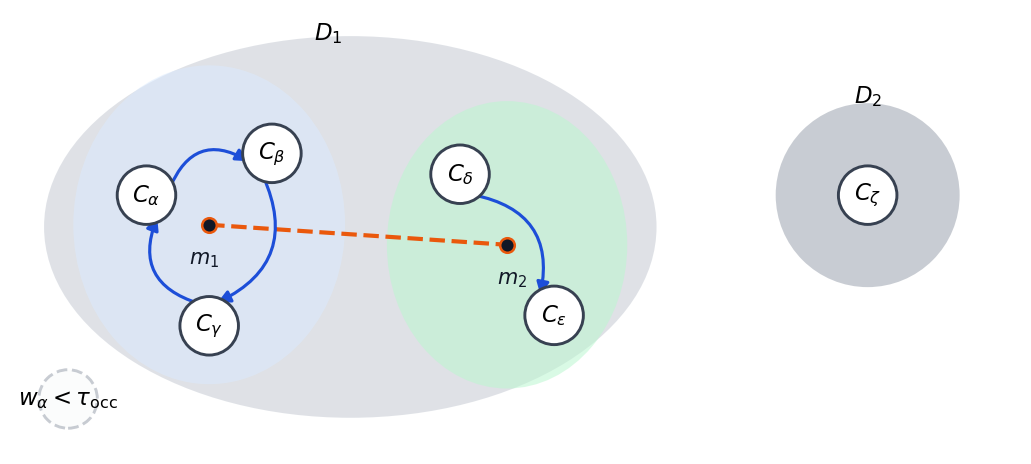
\includegraphics[width=0.95\linewidth]{algorithm/merge_graph_schematic.png}
\caption{Schematic of the two-stage merge procedure. Fine cells $C_\alpha,\ldots,C_\varepsilon$ are first over-partitioned by clustering approximate invariant observables. The blue and green ovals are transition-merged components: cells within each region are connected by frequent one-step transitions (blue arrows, threshold $\tau_{\mathrm{tr}}$). The grey region $D_1$ is then obtained by value-space merging: the orange dashed edge joins the cluster centroids $m_1$ and $m_2$ when $\|m_1-m_2\|_2\le\tau_{\mathrm{val}}$, coarsening the two transition-merged groups into one final component. The separate grey region $D_2$ contains $C_\zeta$. The final partition is $\{D_1,D_2\}$.}
\label{fig:merge_schematic}
\end{figure}


\begin{algorithm}[t]
\caption{Approximating the $\omega$-limit partition}
\label{alg:post_process}
\begin{algorithmic}[1]
\REQUIRE Snapshot pairs $\{(x_i,y_i)\}_{i=1}^N$, dictionary $\Psi=\{\psi_1,\ldots,\psi_s\}$, tolerance $\epsilon$, scalar cluster counts $k_1,\ldots,k_r$, thresholds $\tau_{\text{occ}}$, $\tau_{\text{tr}}$, $\tau_{\text{val}}$.
\STATE Form $M_\Psi$, $N_\Psi$ and solve the GEP \eqref{eq:empirical_GEP}.

\STATE Select eigenvectors $c_1,\ldots,c_r$ satisfying $\lambda\leq\epsilon^2$ and define $f_j(x)=\Psi(x)c_j$ for $j\in[r]$.

\STATE For each $j\in[r]$, cluster $\{f_j(x_i)\}_{i=1}^N$ into $\Ic_1^j,\ldots,\Ic_{k_j}^j$.
\STATE For each $x_i$, compute the multi-index $a(x_i)=(a_1(i),\ldots,a_r(i))$ induced by the scalar clusters.
\STATE Form only the occupied fine cells $\widehat C_\alpha=\{x_i:a(i)=\alpha\}$ for $\alpha\in\mathfrak A=\{a(i):i\in[N]\}$.
\STATE Compute cell weights $w_\alpha=|\widehat C_\alpha|/N$ and embedding centroid $m_\alpha$. Retain cells with $w_\alpha\geq\tau_{\text{occ}}$.

\STATE Build a merge graph with one node per retained fine cell.

\STATE Add edges $(\alpha,\beta)$ based on \eqref{eq:transition_merge_rule} and \eqref{eq:value_merge_rule}.

\STATE Compute the connected components $\mathfrak M_1,\ldots,\mathfrak M_L$.
\STATE Return the final partition $\Pc=\{ \bigcup_{\alpha\in\mathfrak M_\ell} C_\alpha\}_{\ell=1}^L$.
\end{algorithmic}
\end{algorithm}

\section{Simulation Results}
\label{sec:numerical_examples}
We demonstrate the proposed approach on two systems with distinct asymptotic regions. All simulations are performed in Python 3.11.4 on a machine with an Apple M1 Pro chip and 16 GB of RAM. The simulations run in less than a minute including the generalized eigenvalue problem and the post-processing steps.

\subsection{Duffing Oscillator}
Consider the damped Duffing oscillator
\begin{align}
    \dot{x_1} &= x_2, \\
    \dot{x_2} &= -\delta x_2 + \alpha x_1 - \beta x_1^3,
\end{align}
with parameters $\delta = 0.5$, $\alpha = 1.0$, and $\beta = 1.0$. The system has two stable equilibria at $(\pm\sqrt{\alpha/\beta},0)$ and an unstable equilibrium at $(0,0)$. We simulate $500$ trajectories with random initial conditions uniformly in $[-2,2]^2$, sampling every $\Delta t=0.05$ for $100$ time steps ($T=5\,\mathrm{s}$), yielding $N=5\times 10^4$ one-step snapshot pairs. To recover the partition (Algorithm~\ref{alg:post_process}), we use a dictionary of $s=500$ Gaussian RBFs $\phi(r)=\exp(-r^2/2\gamma^2)$ with k-means centers and $\gamma=30$, augmented by the constant function (polynomial degree~$0$). The small RBF support helps approximate nearly piecewise-constant invariant observables. Solving GEP~\eqref{eq:empirical_GEP} with $\epsilon=10^{-4}$ selects two approximate invariant modes, which are clustered with $(k_1,k_2)=(2,4)$ and merged using $\tau_{\mathrm{occ}}=0.002$, $\tau_{\mathrm{tr}}=0.005$, and $\tau_{\mathrm{val}}=0$. This produces two components (Figure~\ref{fig:duffing_results}).

\begin{figure}[htb!]
\centering
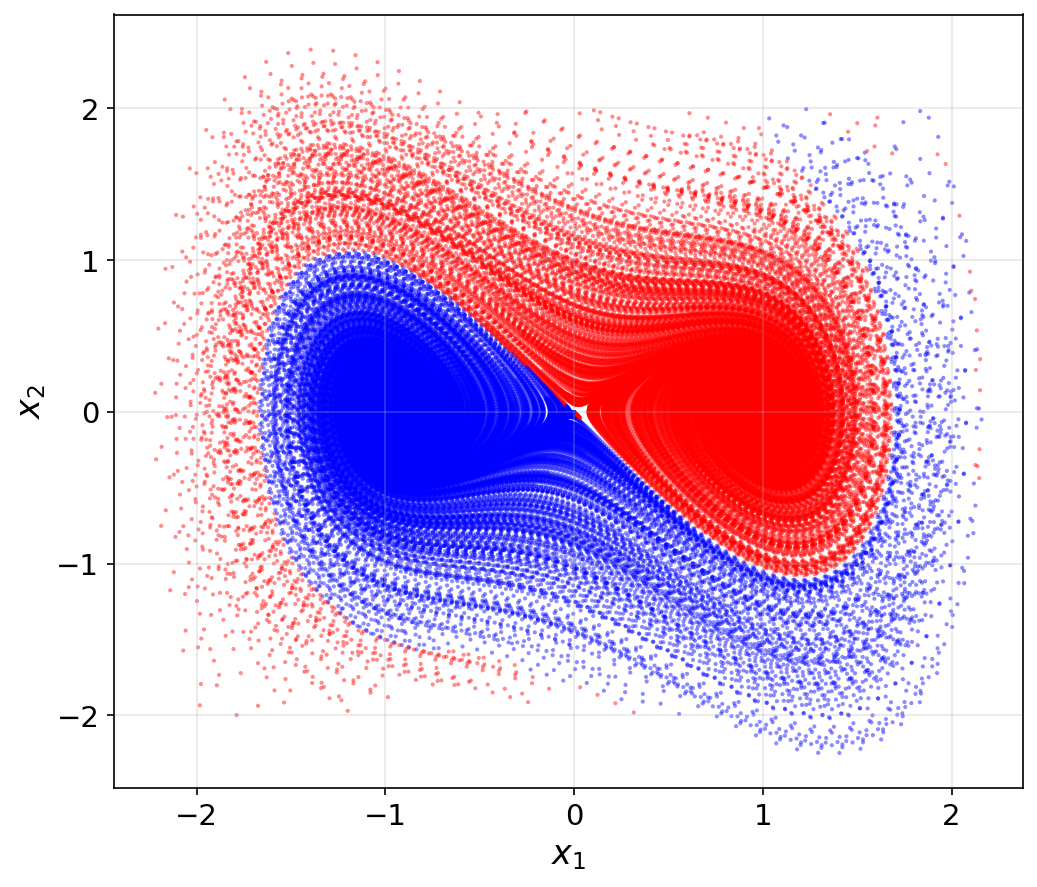
\includegraphics[width=0.95\linewidth]{duffing/multiple_linear_models/partition_scatter.png}
\caption{Recovered $\omega$-limit partition for the Duffing oscillator: training snapshots colored by merged component label.}
  \label{fig:duffing_results}
\end{figure}

Each merged component is used to build a local EDMD model fit on snapshots classified by according to the merged component label. The EDMD dictionary is separate from the partition dictionary and consists of $50$ Gaussian RBF centers subsampled from the training pool, polynomials of degree up to~$3$, and bandwidth $\gamma=10$. For multi-step prediction, an initial condition is classified once against anchors at the stable equilibria $(\pm 1,0)$ and propagated by $\Psi(x_{t+1})\approx \Psi(x_t)K_\ell$ and $x_{t+1}\approx \Psi(x_{t+1})R_\ell$. Figure~\ref{fig:duffing_switched} compares true and predicted trajectories for a few initial conditions; Table~\ref{tab:validation} reports mean relative rollout error on validation trajectories with correctly classified initial conditions.

\begin{figure}[htb!]
\centering
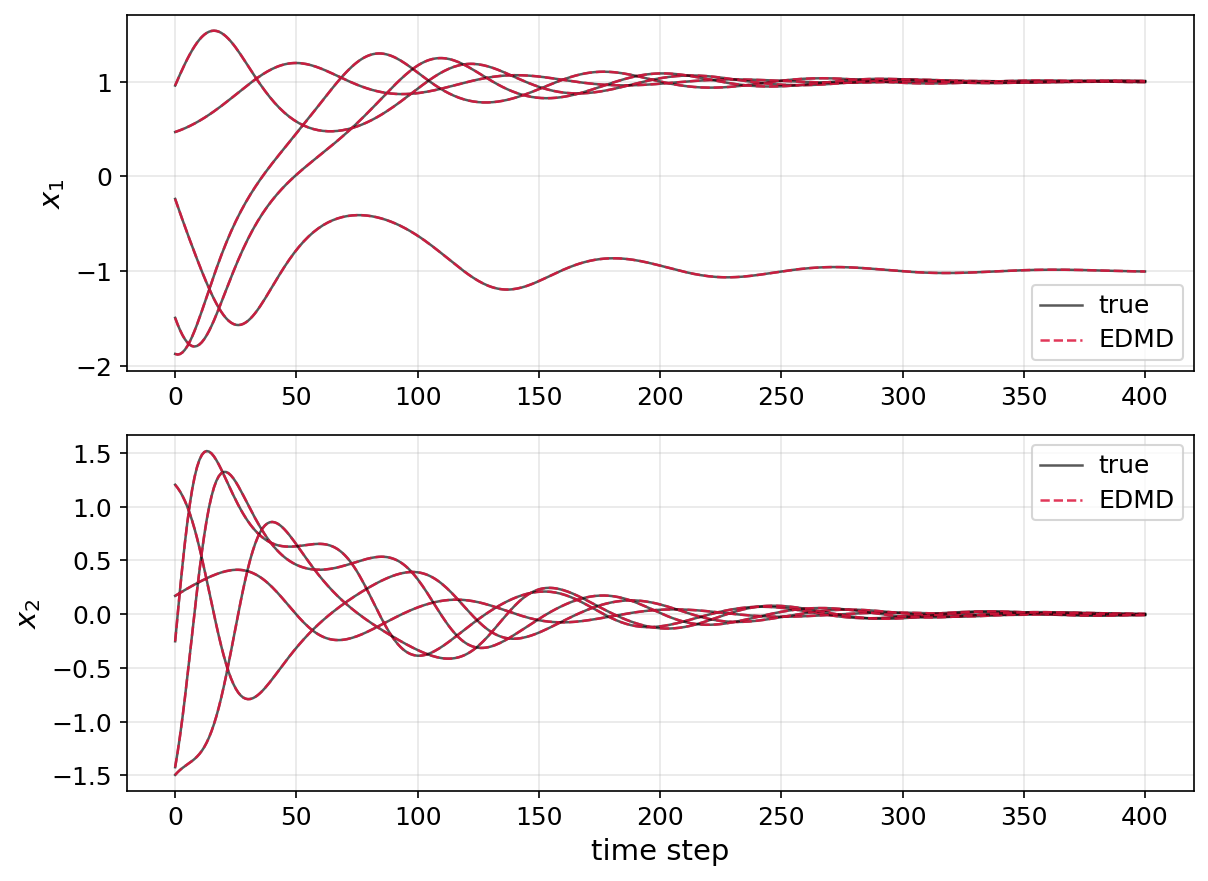
\includegraphics[width=0.95\linewidth]{duffing/multiple_linear_models/phase_trajectories.png}
\caption{Switched local Koopman prediction for the Duffing oscillator: true vs.\ switched-EDMD state trajectories.}
\label{fig:duffing_switched}
\end{figure}

\begin{remark}[Parameter Tuning]
We increase $\gamma$ until the generalized eigenvalue problem produces enough approximate invariant observables with eigenvalues below the prescribed tolerance. We then choose the scalar clustering integers $k_1,\ldots,k_r$. In practice, the parity of $k_j$ can affect the quality of the initial fine partition. For the merging thresholds, we tune the transition threshold $\tau_{\mathrm{tr}}$ before using value-space merging. Specifically, we first set $\tau_{\mathrm{val}}=0$ so that merging is driven only by observed transitions between fine cells. We then vary $\tau_{\mathrm{tr}}$. Smaller values of $\tau_{\mathrm{tr}}$ produce more aggressive merging and, in the extreme, may collapse the partition to a single cell. Starting from a small value, we gradually increase $\tau_{\mathrm{tr}}$ until persistent cells appear and the resulting partition is approximately stationary on the data. After $\tau_{\mathrm{tr}}$ is fixed, the value-space threshold $\tau_{\mathrm{val}}$ can be used as a secondary refinement parameter. In our experiments, transition-based merging was often sufficient, and $\tau_{\mathrm{val}}$ was needed only for fine-tuning. 
\end{remark}

\subsection{Bistable Oscillations}
Consider the bistable oscillation model in polar coordinates:
\begin{align}
    \dot{r} &= (r - 2) - (r - 2)^3, \\
    \dot{\theta} &= 1.
\end{align}

This system has two stable limit cycles at $r = 1, 3$ and an unstable limit cycle at $r = 2$. We convert the polar coordinates to Cartesian coordinates for analysis. We simulate $500$ trajectories with random initial conditions uniformly in $[0,4]\times[0,2\pi]$, sampling every $\Delta t=0.05$ for $51$ time steps ($T=2.5\,\mathrm{s}$), yielding $N=2.5\times 10^4$ snapshot pairs. The partition is computed with $s=500$ k-means RBF centers, polynomials of degree up to~$3$, and $\gamma=1$. GEP~\eqref{eq:empirical_GEP} with $\epsilon=10^{-4}$ yields four approximate invariant modes. Algorithm~\ref{alg:post_process} is applied with $(k_1,k_2,k_3,k_4)=(1,4,4,2)$ and $(\tau_{\mathrm{occ}},\tau_{\mathrm{tr}},\tau_{\mathrm{val}})=(8\times 10^{-4},\,0.1,\,7\times 10^{-6})$, producing two merged limit-cycle components (Figure~\ref{fig:bistable_results}).

\begin{figure}[htb!]
\centering
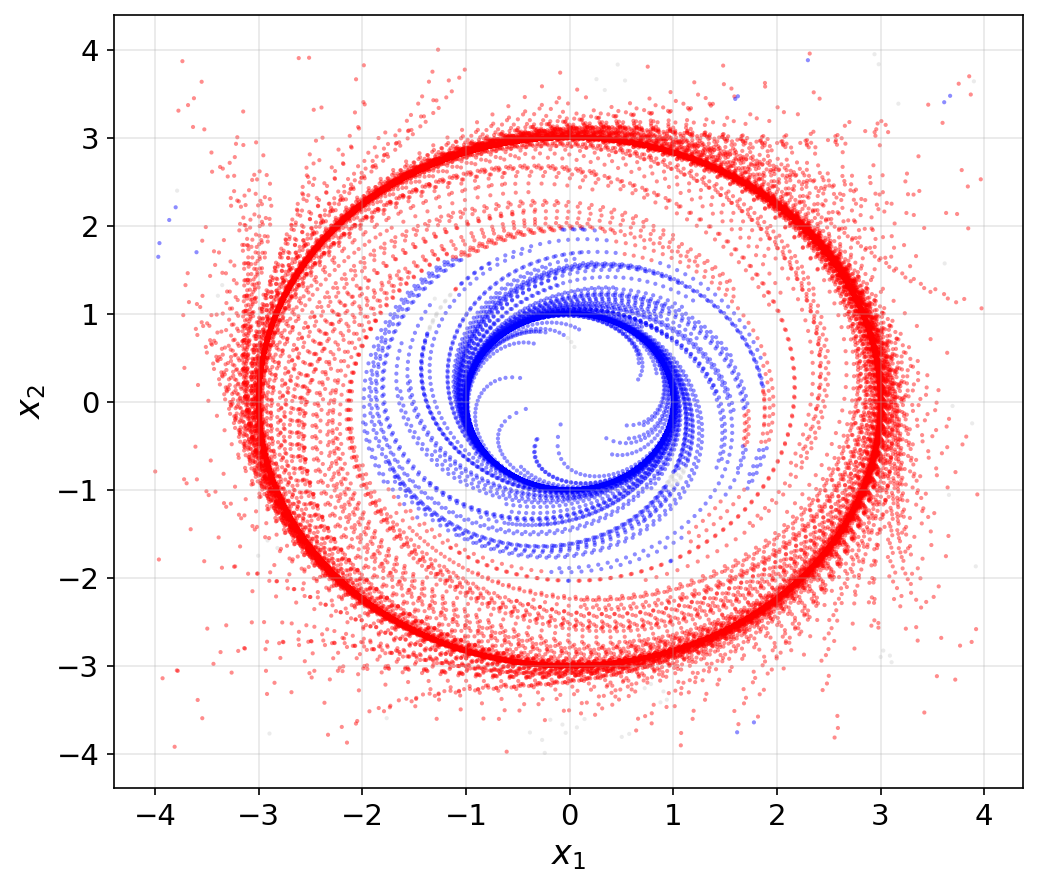
\includegraphics[width=0.95\linewidth]{bistable_oscillations/multiple_linear_models/partition_scatter.png}
\caption{Recovered $\omega$-limit partition for the bistable oscillations: training snapshots colored by merged component label.}
  \label{fig:bistable_results}
\end{figure}

Local EDMD models on each component use a separate dictionary consisting of $10$ RBF centers subsampled from the training pool, polynomials of degree up to~$3$, and $\gamma=1$. Classification anchors are representative snapshots on the inner and outer limit cycles. Figure~\ref{fig:bistable_switched} compares true and switched trajectories for four prescribed initial conditions. Rollout errors in Table~\ref{tab:validation} are computed as in the Duffing example, using only trajectories with correctly classified initial conditions.

\begin{figure}[htb!]
\centering
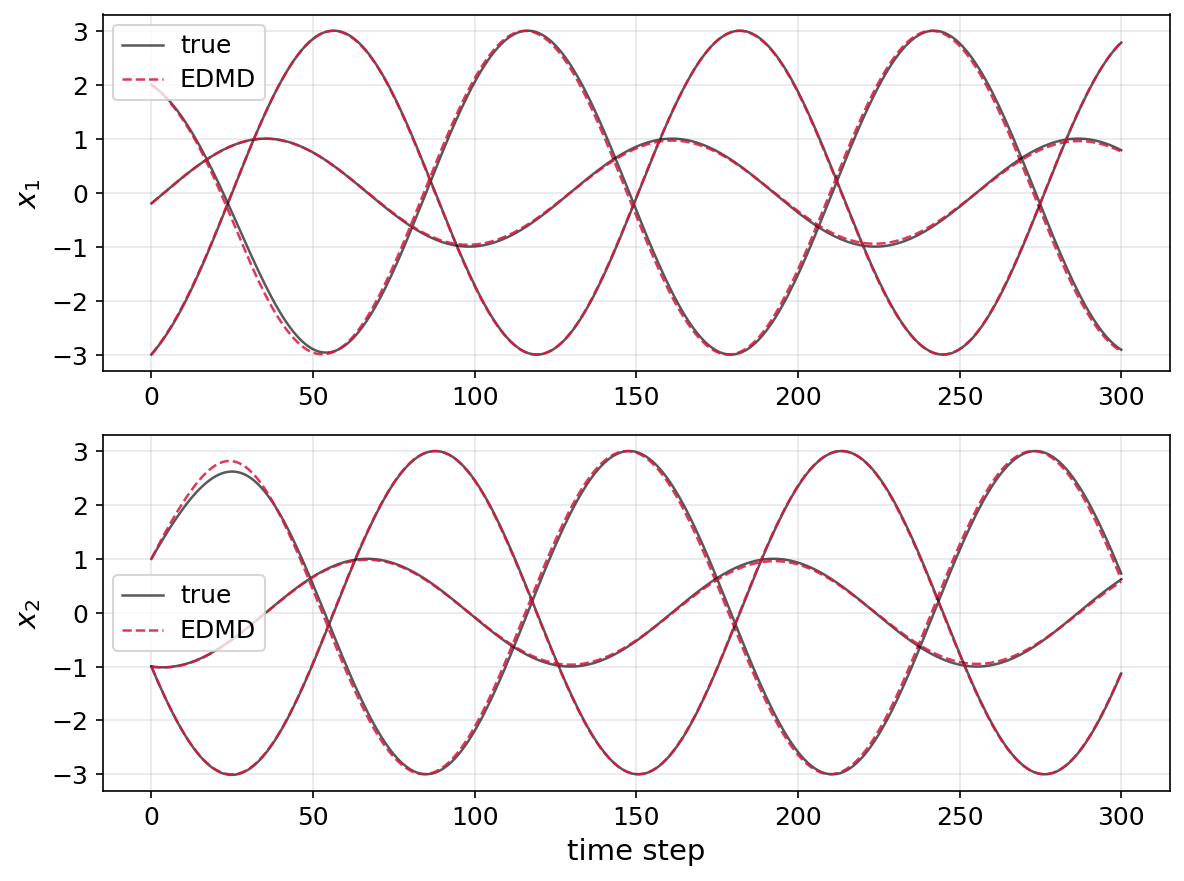
\includegraphics[width=0.95\linewidth]{bistable_oscillations/multiple_linear_models/phase_trajectories.png}
\caption{Switched local Koopman prediction for the bistable oscillations: true vs.\ switched-EDMD state trajectories.}
\label{fig:bistable_switched}
\end{figure}

Table~\ref{tab:validation} summarizes partition classification accuracy and mean relative rollout error $\|\hat{x}_t-x_t\|/\|x_t\|$ at selected time steps on trajectories with correctly classified initial conditions. Together, the qualitative and quantitative results show that recovering the $\omega$-limit partition enables component-wise Koopman models that preserve distinct asymptotic behaviors and remain accurate over long horizons when the initial classification is correct.

\begin{table}[htb!]
\centering
\resizebox{\linewidth}{!}{%
\begin{tabular}{@{}lcccccc@{}}
\toprule
System & Accuracy & $t\!=\!0$ & $t\!=\!50$ & $t\!=\!100$ & $t\!=\!200$ & $t\!=\!300$ \\
\midrule
Duffing & 99.86\% & $0$ & $3.8\!\times\!10^{-4}$ & $3.8\!\times\!10^{-4}$ & $1.2\!\times\!10^{-4}$ & $5.0\!\times\!10^{-5}$ \\
Bistable osc. & 99.80\% & $0$ & $5.1\!\times\!10^{-2}$ & $3.5\!\times\!10^{-2}$ & $1.9\!\times\!10^{-2}$ & $2.1\!\times\!10^{-2}$ \\
\bottomrule
\end{tabular}%
}
\caption{Classification accuracy of the recovered $\omega$-limit partition is reported on validation data. Other columns report mean relative state error averaged over several trajectories at time step $t$ for correctly classified initial conditions.}
\label{tab:validation}
\end{table}

\section{Conclusion}
This paper addressed the recovery of omega-limit partitions for autonomous systems with multiple asymptotic behaviors. For data-driven settings, we proved that approximate invariant observables obtained from a finite dictionary can create a refinement of the omega-limit partition outside a small exceptional set when the dictionary approximates cell indicators, thereby motivating a post-processing merging strategy for partition recovery.

Building on this theory, we developed a practical procedure that solves a generalized eigenvalue problem for approximate invariant modes, clusters snapshot data in the resulting embedding, and merges fine cells using transition- and value-space criteria (Algorithm~\ref{alg:post_process}). The merged partition supports multiple local EDMD models fit independently on each component. On the Duffing oscillator and a bistable limit-cycle example, the method recovered the expected asymptotic regions with classification accuracy above $99.8\%$ and enabled long-horizon prediction that respects distinct omega-limit behaviors when initial conditions are correctly classified.

These results suggest a constructive alternative to a single global Koopman model in settings where multiple omega-limit sets obstruct continuous finite-dimensional embeddings. Important open directions include dictionary and threshold selection for higher-dimensional systems, online or adaptive reclassification during rollout, finite-sample performance guarantees, and the integration of recovered partitions into analysis and control design with discontinuous Koopman representations.

\bibliographystyle{ieeetr}
\bibliography{\biblink/alias,\biblink/Main-add,\biblink/Main,\biblink/JC}



\end{document}

% section titles
% prop titles
